%
% Complete documentation on the extended LaTeX markup used for Insight
% documentation is available in ``Documenting Insight'', which is part
% of the standard documentation for Insight.  It may be found online
% at:
%
%     http://www.itk.org/

\documentclass{InsightArticle}

\usepackage[dvips]{graphicx}

%%%%%%%%%%%%%%%%%%%%%%%%%%%%%%%%%%%%%%%%%%%%%%%%%%%%%%%%%%%%%%%%%%
%
%  hyperref should be the last package to be loaded.
%
%%%%%%%%%%%%%%%%%%%%%%%%%%%%%%%%%%%%%%%%%%%%%%%%%%%%%%%%%%%%%%%%%%
\usepackage[dvips,
bookmarks,
bookmarksopen,
backref,
colorlinks,linkcolor={blue},citecolor={blue},urlcolor={blue},
]{hyperref}
\usepackage{subfigure}

%  This is a template for Papers to the Insight Journal. 
%  It is comparable to a technical report format.

% The title should be descriptive enough for people to be able to find
% the relevant document. 
\title{Implementation of a 3D thinning algorithm}

% Increment the release number whenever significant changes are made.
% The author and/or editor can define 'significant' however they like.
\release{1.00}

% At minimum, give your name and an email address.  You can include a
% snail-mail address if you like.
\author{Hanno Homann$^{1}$}
\authoraddress{$^{1}$Oxford University, Wolfson Medical Vision Lab}

\usepackage{setspace}
\onehalfspacing

\begin{document}


\ifpdf
\else
   %
   % Commands for including Graphics when using latex
   % 
   \DeclareGraphicsExtensions{.eps,.jpg,.gif,.tiff,.bmp,.png}
   \DeclareGraphicsRule{.jpg}{eps}{.jpg.bb}{`convert #1 eps:-}
   \DeclareGraphicsRule{.gif}{eps}{.gif.bb}{`convert #1 eps:-}
   \DeclareGraphicsRule{.tiff}{eps}{.tiff.bb}{`convert #1 eps:-}
   \DeclareGraphicsRule{.bmp}{eps}{.bmp.bb}{`convert #1 eps:-}
   \DeclareGraphicsRule{.png}{eps}{.png.bb}{`convert #1 eps:-}
\fi


\maketitle


\ifhtml
\chapter*{Front Matter\label{front}}
\fi


% The abstract should be a paragraph or two long, and describe the
% scope of the document.
\begin{abstract}
\noindent

ITK currently comes with a 2D binary thinning (skeletonisation) method, but does not support 3D or higher. This paper documents a new \texttt{itkBinaryThinningImageFilter3D} and recommends to rename the current filter as \texttt{itkBinaryThinningImageFilter2D}.

The 3D method suggested here is a direct implementation of the work of Lee et al.~\cite{lee1994bsm} who have demonstrated that their algorithm can find all deletable surface points at every iteration and is thus very fast. The code was tested on six clinical datasets.
\end{abstract}

\tableofcontents


\section{Introduction}

Binary thinning is used for finding the centrelines ("skeleton") of objects in the input image. The general idea is to erode the object's surface iteratively until only the skeleton remains.
Erosion has to be performed symetrically in order to the guarantee medial position of the skeleton lines and such that the connectedness of the object is preserved. Care has to be taken in order not to create holes or cavities in the object.

There are two major approaches to image thinning: a) kernel-based filters and b) decision trees.
Kernel-based filters apply a structuring element to the image and can generally be extented to dimensions higher than 3D (see e.g.~\cite{jonker1953moa}), to find computationally efficient solutions for 4D and higher dimensions is subject of ongoing research.
Methods based on decision trees are thus far limited to 2D and 3D, but are potentially faster than morphological filters, if they are well designed and can find more deletable points at each iteration.

In 3D there are $2^{26} = 67,108,864$ possible binary combinations of object and background voxels in a 26-neighbourhood, which cannot be completely captured by kernel-based filters. 
Lee et al.~have demonstarted in their work  \cite{lee1994bsm} that their solution, based on a decision tree, can handle all these cases correctly and find \textit{all} deletable surface points at each iteration. Thus their algorithm allows for a very fast iterative erosion process and was chosen for the implementation presented in this paper.

Currently ITK comes with the \texttt{itkBinaryThinningImageFilter} for skeletonisation of 2D images, based on a decision tree. However, ITK does not yet contain a method that can handle 3D thinning.
Since a 2D and a 3D thinning filter based on decision trees demand for distinct implementations, the author suggestes to rename ITK's current \texttt{itkBinaryThinningImageFilter} as \texttt{itkBinaryThinningImageFilter2D} and to add a new method named \texttt{itkBinaryThinningImageFilter3D} which is described below.

\section{Method}
The new 3D method is documented here and contains of a prepcocessing stage and an implementation of Lee's algorithm \cite{lee1994bsm}. Apart from the input and output image type, no user-defined paramters are required.

At the preprocessing stage, our function \texttt{PrepareData()} transforms the input image to a binary image by setting all non-zero valued pixels to one. This is done in the same way as in the \texttt{itkBinaryThinningImageFilter(2D)}.

At the main stage, our function \texttt{ComputeThinImage()} performs a number of tests in order to check if a pixel can be eroded from the object. This is done for all pixels in the image and repeated until no more change occurs. The current pixel can be deleted:

\begin{enumerate}
	\item if the current pixel is a surface pixel. This test only considers one the six possible directions in 3D at a time in order to perform thinning symmetrically, i.e. to guarantee that the centrelines are not shifted to one side of the object.
	\item if the pixel is not the end of a line, because the centre lines are to remain.
	\item if the deletion of the point would not change the Euler characteristic, i.e.~if no holes are created when deleting the pixel. This is done by using the look-up table (LUT) from~\cite{lee1994bsm}.
	\item if the current point is a \textsl{simple point}, that is it's deletion does not change the number of connected objects. This test is performed last as it's the computationally most expensive one.
\end{enumerate}

Details about the Euler invariance and the connected components check can be found Lee's paper,  which the provided code strictly follows. The algorithm uses 26-neighbourhood connectivity for the object and 6-neighbourhood connectivity for the background and guarantees unchanged connectedness of the objects as well as not to create holes or cavities in the object. The output of the algorithm is a binary image that contains only the centrelines, marked as "`\texttt{1}"'. 

All these tests are performed in parallel to all voxels of the 3D image, but multi-threading has not been implemented, yet. Finally, a sequential re-checking method is required to ensure that connectivity is preserved even after deletion of neighbour voxels, as suggested by Lee.


\section{Results}
The 3D thinning algorithm has been successfully tested on segmentations of the hepatic vasculature from six clinical datasets. In each case the image size was about $300x300x40$ and the computation was finished within a few seconds on a standard PC. An example is given in figure~\ref{fig:results-thinning}, showing the original 3D object on the left and a projection of the filter output on the right.

Visual scrutiny showed that, despite of the complexity and the noisy surfaces of the input object, the output of the filter well meets our expectations: Connectivity is preserved and the skeleton lines are well located in the centre of the object.

In this case the skeleton image contains a blob-like structure (arrow) which is due to a cavity in the original object which is preserved and eroded from the inside by the algorithm.

\begin{center}%
\begin{figure}[h]%
\begin{centering}
\subfigure[Surface rendering of the original 3D object (Hepatic vasculature segmentation)]{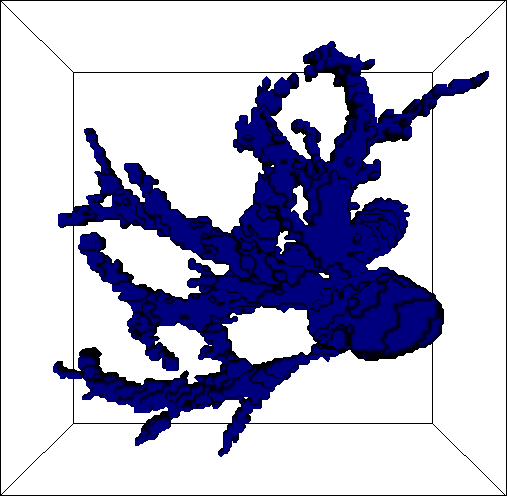
\includegraphics[width=0.45\textwidth]{images/segmentation}}
\hspace{0.05\textwidth}%
\subfigure[Projection of its skeleton after thinning]{
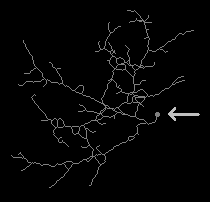
\includegraphics[width=0.45\textwidth]{images/skeleton}}
\par%
\end{centering}
\caption{Comparison of an object and its skeleton.\label{fig:results-thinning} }
\end{figure}
\par\end{center}

\section{Conclusions}
The 3D thinning algorithm presented by Lee et al.~, based on a decision tree, allows for very fast image thinning as it can find all deletable surface points at each iteration. We implemented their  method for ITK as \texttt{itkBinaryThinningImageFilter3D}, tested our code on six 3D binary images with complex vascular objects and found that the algorithm performs reliably and fast.

Lee's method is a parallel method, thus adding multi-threading capabilities to our code might improve performance.

%%%%%%%%%%%%%%%%%%%%%%%%%%%%%%%%%%%%%%%%%
%
%  Insert the bibliography using BibTeX
%
%%%%%%%%%%%%%%%%%%%%%%%%%%%%%%%%%%%%%%%%%

\bibliographystyle{plain}
\bibliography{InsightJournal}


\end{document}

